\documentclass{article}
\usepackage{graphicx}
\usepackage{subfiles}
\usepackage{subfigure}
\usepackage{color}
\usepackage[hidelinks]{hyperref}
\graphicspath{{pics/}}

\title{Traitement numérique du signal \\ \vspace{5mm} Livrable final \\ \vspace{3mm} Groupe G10C } 
\author{MANGIN Rémi \\
LE MONNIER Romain \\
TEOFILOVIC Kristina \\
TON Sophie \\
RISY Théo \\
YANG Chen}   
\date{\today}  
\begin{document}

\maketitle

\newpage
\tableofcontents
\newpage

\textbf{Problème II :} \  \\
Proposer un algorithme qui permet de détecter, de caractériser une note de musique jouée par un instrument (violon, flûte, piano) et de déterminer sa hauteur. \\
Cet algorithme devra produire les sorties suivantes : \\
\begin{itemize}
    \item $t_d, t_f$: instants de début et de fin de note
    \item $P_dBm$: la puissance moyenne du signal en dBm
    \item $f_0$: la fréquence fondamentale et le nom et l'octave de la note jouée
    \item $f_h$: la fréquence haute telle que [0,$f_h$] contient 99.99\% de la puissance
    \item $n_h$: le nombre d'harmoniques dans cette bande de fréquences
    \item Toutes autres caractéristiques qui vous paraît pertinente pour classifier les notes par instrument de musique.
    On reprendra la méthode de détection d'un son utile du PBI et on justifiera les paramètres retenus.
\end{itemize}

\textbf{Problème IV :} \ \\
On souhaite détecter les signaux environnementaux qui comprennent des composantes spectrales très aiguës et pénibles pour l'oreille humaine. Ces signaux sont définis ainsi : 20\% de leur puissance est comprise dans les fréquences supérieures à 2 kHz, avec une puissance sonore totale supérieure à 110 dB SLP. \\
Concevoir un système de détection de ces signaux pénibles fondé sur filtrage
numérique. On prendra un micro de sensibilité égale à -67 dBV et de gain égal à 16 dB. Discuter les critères énoncés.

  
\newpage
\textcolor{blue}{\section{Chapitre I : Problème I}}
\textcolor{blue}{\subsection{Introduction}}
Nous présentons une approche de détection de signaux audio , dont les caractéristiques sont les suivantes :
\begin{itemize}
    \item Un micro avec une sensibilité (S) de - 48 dBV et un Gain (G) de 40 dB.
    \item Les sons pénibles sont définis comme des sons de plus d'une seconde, dépassant une puissance en dBm de référence.
    \item Les sons acceptables sont définis en dessous de ce seuil.
    \item Chaque signal sera caractérisé par sa durée, sa puissance moyenne, tension RMS, et classifié en conséquence. 
\end{itemize}

Les expérimentations seront réalisées sur les signaux de la question F, signaux qui nous ont été fournis (bruit de marteau piqueurs, bruit de ville et de jardin). Dans un premier temps, nous implémenterons le code de détection sur le micro-contrôleur, en choisissant une fréquence d'échantillonnage adaptée aux caractéristiques matérielles. La caractérisation des bruits détectés fera l'objet d'une étape ultérieure.
\newline 
\\
 \textbf{Problème I - Énoncé } \ \\
Proposer un algorithme qui permet de détecter la présence/absence d’un signal audio enregistrant le bruit ambiant.
Le micro utilisé a une sensibilité S (dBV) et amplifie le signal électrique avec un gain G. On définit un son "son pénible", comme un signal sonore de durée supérieure à Dt (s) et de niveau supérieur ou égal à $P_{SPL}$ (dB SPL1). A contrario, un "son acceptable", correspond à un signal sonore de niveau inférieur à $P_{SPL}$.
\\
Caractériser chaque son détecté par :
\begin{itemize}
    \item Sa durée 
    \item sa puissance
    \item sa tension RMS en V et le classifier en "son pénible" ou "son acceptable"
\end{itemize}
Paramètres S = -48 dBV, G = 40 dB, $P_{SPL}$ = 80 dB SPL, $D_t$ = 1s.
\\
Les expérimentations seront menées sur les signaux de la question F.








\textcolor{blue}{\subsection{Méthode}}Tout d'abord, il faut définir $P_{dBm}$. Le schéma du microphone qui nous est donné permet de réaliser les calculs.

\begin{figure}[htb]
    \centering
    \includegraphics[width=0.8\textwidth]{schemabloc_méthode1.png}
    \caption{Schéma bloc microphone}
    \label{fig:Schéma_Fonctionnel_1}
\end{figure}

En effet, nous avons la relation suivante :
\begin{equation}
P_{dBm} = 10 \times \log(V_a^2 \times 1000) \ \text{avec}\ V_a = S \times P_a
\end{equation}
Cependant, S la sensibilité \footnote{\href{http://electroacoustique.univ-lemans.fr/cours/Grain1.2/co/grain2_2_2.html}{Pour la formule de la sensibilité S}} que l'on nous donne est en dBV et pas en $V/P_a$, il faut donc la convertir. Nous savons que :\begin{equation}
    S = 20\times \log(\frac{S_{v/Pa}}{S_{ref}}) \ \text{avec}\  S_{ref} = 1 V/P_a
\end{equation} donc :
\begin{equation}
   S_{V/P_a} = S_{ref}*10^\frac{S}{20} 
\end{equation}
Nous avons donc :
\begin{equation}
V_m = S_{V/P_a} \times P_a
\end{equation} 
Pour $P_a$, nous utilisons la formule de $P_{SPL}$ \footnote{\href{https://fr.wikipedia.org/wiki/Pression_acoustique}{Pour la formule de $P_{SPL}$}}: 
\begin{equation}
    P_{SPL} = 20\times \log(\frac{P_a}{P_{ref}}) 
\end{equation}
d'où :
\begin{equation}
P_a = P_{ref} * 10^{\frac{P_{SPL}}{20}}
\end{equation}
Il ne reste que le gain à traiter, celui-ci s'exprime en dB dans les paramètres donnés, or, nous voulons l'exprimer sans unité, nous obtenons alors 
\begin{equation}
    G_{SU} = 10^\frac{G}{20} \ \text{où} \ G_{SU} \ \text{est sans unité} \footnote{\href{https://fr.wikipedia.org/wiki/Gain_d\%C3\%A9cibel}{Pour la formule du gain sans unité $G_{SU}$}}
\end{equation}

Cela nous permet de trouver la formule finale : 
\\
\tcbox[colback=yellow!20, colframe=yellow, boxrule=2pt]{$ P_{dBm} = 10 \times \log((G_{SU} \times S_{VPA} \times P_a)^2 \times 1000)$}

En substituant avec les résultats précédents, on obtient :
\tcbox[colback=green!20, colframe=green, boxrule=2pt]{$P_{dBm} = 20 \times \log(10^\frac{G}{20} \times S_{REF} \times 10^{\frac{S}{20}} \times P_{REF} \times 10^{\frac{P_{SPL}}{20}})+30$}
Enfin, avec : \begin{itemize}
    \item $S_{REF} = 1$
    \item $P_{REF} = 20 \mu Pa$
    \item $G = 40 dB$
    \item $S = -48 dBV$
    \item $P_{SPL} = 80 dB SPL$
\end{itemize} 
On obtient : \tcbox[colback=green!20, colframe=green, boxrule=2pt]{$P_{dBm} = 8 dBm$.}
À présent, nous avons la valeur de $P_{dBm}$ qui va nous servir de référence. Pour chaque signal, nous allons le décomposer en plusieurs « sous-signaux » à chaque fois que la valeur de référence est franchie. 
Par exemple, sur la figure \ref{Fig.1.2}, on distingue trois « sous-signaux » ou plages de signal différentes, car la valeur de référence est franchie deux fois. Ensuite, chaque plage est traitée comme un nouveau signal et, si cette plage se trouve au-dessus de la valeur référence et dure plus d’une seconde, alors le son de cette plage est catalogué dans la catégorie bruit pénible. Sur cet exemple, il y a donc deux sons acceptables (plages 1,3) et un son pénible (plage 2).
Enfin, pour chaque signal, on règle la taille des fenêtres d’analyse pour obtenir un résultat correct, contenant 2k+1 échantillons.Pour déterminer la puissance instantanée, nous utilisons la formule suivante :
\begin{equation}
    P(n) = \frac{1}{2K+1}\sum_{n-K}^{n+K}_{x(k)^2}
\end{equation}
L'identification du paramètre k ainsi que le choix de sa valeur retenue dépendent de la nature du signal et des exigences spécifiques de l'analyse. Admettons que nous avons un signal de 5s et d'une fréquence de 20k Hz, si k = 80, on aura 161 échantillons par fenêtre. Pour un signal sonore, il faut que la taille de la fenêtre soit petite, car c'est un fichier son. Pour avoir un bon vecteur puissance à analyser, il faut donc une fenêtre inférieure à la seconde, comme on a Te, il faut déterminer k tel que :
\begin{equation}
    k < \frac{(\frac{1}{Te}-1)}{2}
\end{equation}
\begin{figure}[htb]
    \centering
    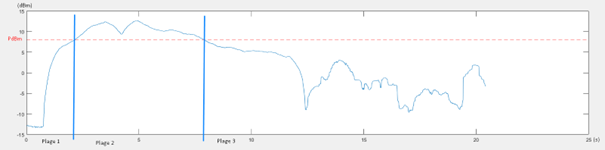
\includegraphics[width=0.8\textwidth]{Exemple_seuil_se_pénibilité.png}
    \caption{Exemple signal avec plages acceptables et pénibles}
    \label{Fig.1.2}
\end{figure}


\textcolor{blue}{\subsection{Résultats Expérimentaux}}
Après avoir appliqué la fonction du problème aux signaux Jardin01.mp3, Jardin02.mp3, Ville01.mp3 et MarteauPiqueur01.mp3, voici ce que nous obtenons :
\\
\\
\textbf{Légende :}
\\
\textcolor{red}{Rouge :} dépasse la durée et la puissance seuil
\\
\textcolor{blue}{Bleu : }dépasse la puissance seuil, mais plus petit que dt

\begin{figure}[htb]
\subfigure[Application sur le signal Jardin01]{
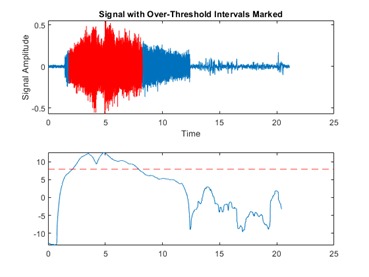
\includegraphics[width = 0.45\textwidth]{jardin01.png}
\label{Fig.sub.1.3.1}
}
\subfigure[Application sur le signal Jardin02]{
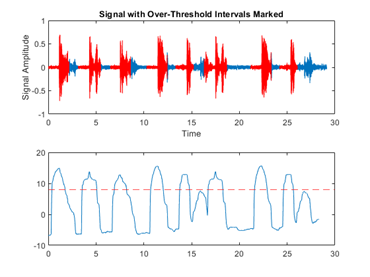
\includegraphics[width = 0.45\textwidth]{jardin02.png}
\label{Fig.sub.1.3.2}
}
\subfigure[Application sur le signal MarteauPiqueur]{
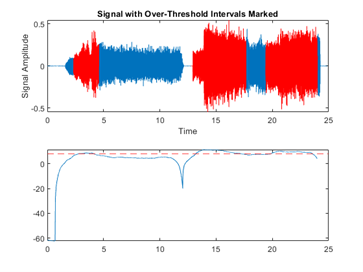
\includegraphics[width = 0.45\textwidth]{marteaaupiqueur01.png}
\label{Fig.sub.1.3.3}
}
\subfigure[Application sur le signal Ville01]{
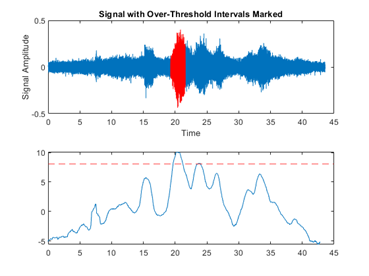
\includegraphics[width = 0.45\textwidth]{ville01.png}
\label{Fig.sub.1.3.4}
}
\caption{Application sur les signaux donnés}
\label{Fig.main.2}
\end{figure}

Pour chacun des signaux, l'amplitude en fonction du temps est présentée en haut, tandis que la puissance en dBm en fonction du temps est affichée en bas. Les pointillés rouges désignent la puissance de référence à 8 dBm et nous observons bien que lorsque le signal dépasse 8 dBm et dure plus d'une seconde, nous avons une plage de son pénible (en rouge).
\\
\\
\begin{table}
  \centering
  \begin{tabular}{|c|c|c|c|c|}
    \hline
    & Ville01 & MarteauPiqueur01 & Jardin01 & Jardin02 \\
    \hline
    Puissance moyenne (dBm) &-27.363 & -22.7752 
  &-23.5662 & -21.5499\\
    \hline
    Puissance moyenne (mW) & 1.835 & 5.2781\times 10^-6 & 4.3992\times10^-6 & 6.9986\times10^-6\\
    \hline
    Durée & 43.5566 & 24.8176 & 21.058 & 29.0993\\
    \hline
    Tension RMS (V) & 0.0013547 & 0.0022974 & 0.0020974 & 0.0026455 \\
    \hline
  \end{tabular}
    \caption{Avant Amplification}
\end{table}
\\
\begin{table}
  \centering
  \begin{tabular}{|c|c|c|c|c|}
    \hline
    & Ville01 & MarteauPiqueur01 & Jardin01 & Jardin02 \\
    \hline
    Puissance moyenne (dBm) & 12.637 & 17.2248 & 16.4338 & 18.4501\\
    \hline
    Puissance moyenne (mW) & 0.018353 & 0.052781 & 0.043992& 0.069986\\
    \hline
    Durée (s)& 43.5566 & 24.8176 & 21.058 & 29.0993 \\
    \hline
    Tension RMS (V) & 0.13547 & 0.22974 & 0.20974 & 0.26455 \\
    \hline
  \end{tabular}
    \caption{Après Amplification}
\end{table}
\\
\newpage
% analyse des sons par rapport au ressenti à l'oreille sons pénible par rapport aux programme 
Dans ce tableau des caractéristiques des différents signaux, nous avons déterminé la puissance moyenne. Elle mesure la puissance d'un signal sur une période de temps donnée et elle est définie comme la quantité totale d'énergie transférée ou consommée divisée par la durée de cette période. Entre deux instants, elle est l'énergie dissipée par la durée d'observation et sa formule est : 
\begin{equation}
    P(x, t_{1}, t_{2}) = \frac{1}{t_{2} - t{1}} \int_{t_{1}}^{t_{2}}x_{c}(t)^2 dt
\end{equation}
\textcolor{blue}{\subsection{Conclusion}}
Pour conclure, le problème 1 a été abordé à travers la conception d’un algorithme dédié à la détection de la présence ou de l’absence de signaux audio, enregistrant ainsi le bruit ambiant. Nos expérimentations ont débuté en utilisant des sons préalablement définis, fournis dans la question F, tels que des bruits de marteau-piqueur, de ville, et de jardin 1 et 2. L’analyse approfondie de ces sons a permis de classer les signaux en deux catégories distinctes : les "sons pénibles", identifiés en rouge, définis par une durée excédant à 1 seconde et une puissance en dBm égale ou supérieure à 8, et les "sons acceptables" distingués en bleu, caractérisés par une puissance en dBm inférieure à ce seuil. 
\\

Nos résultats présentent des points forts notables. La méthode de classification des signaux a démontré une clarté visuelle, facilitée par l'utilisation de couleurs, renforçant ainsi la compréhension des différentes catégories. De plus, la caractérisation détaillée de chaque signal fournit une base solide pour évaluer l'impact des sons sur l'environnement.
\\

Cependant, des points faibles nécessitent une attention particulière. La détermination du seuil de puissance pour les "sons pénibles" pourrait être améliorée pour refléter davantage la variabilité des environnements sonores. De plus, la limitation actuelle de nos expérimentations à des enregistrements préétablis soulève des questions sur la généralisation de notre algorithme à des situations en temps réel et dynamique.
\\

Pour perfectionner notre recherche, nous envisageons d'optimiser la calibration du seuil de puissance en tenant compte de la variabilité environnementale. L'extension de nos expérimentations à des conditions réelles d'environnement sonore permettra une validation plus approfondie de notre algorithme. Ces perspectives d'amélioration visent à renforcer la fiabilité et l'applicabilité de notre méthode dans des situations plus diversifiées et changeantes.

\textcolor{blue}{\section{Chapitre II : Problème II}}
\textcolor{blue}{\subsection{Introduction}}
Nous proposons une approche novatrice visant à élaborer un algorithme de détection et de caractérisation des notes de musique jouées par divers instruments tels que le violon, la flûte et le piano, tout en déterminant précisément leur hauteur. Notre algorithme est conçu pour générer des sorties exhaustives, incluant les instants de début et de fin de chaque note ($t_d$,$t_f$), la puissance moyenne du signal en dBm ($P_{dBm}$), la fréquence fondamentale ($f_0$) accompagnée du nom et de l’octave de la note jouée, la fréquence haute $f_h$ définie par [0, $f_h$] englobant 99.99\% de la puissance, le nombre d’harmoniques dans cette bande de fréquences ($n_h$), ainsi que toute autre caractéristique jugée pertinente pour classifier les notes selon l'instrument de musique. Nous adopterons la méthode de détection d’un son utile du PBI (Produit de l'analyse du Bruit Instantané) pour élaborer notre algorithme, en nous appuyant sur une approche en trois étapes. Cette méthodologie implique la détection du signal sonore, la synchronisation du récepteur par la détection de l'en-tête, et enfin, le décodage des informations pertinentes pour caractériser chaque note. 

\textcolor{blue}{\subsection{Méthode}}

Les signaux originales sont en stéréo, il faut les moyenner pour retrouver dans le cadre du cours.
fig.\ref{Fig.sub.1} est le signal avant moyenner, fig.\ref{Fig.sub.2} est le signal après moyenner.
\begin{figure}[htb]
\subfigure[Exemple de signal audio original]{
\label{Fig.sub.1}
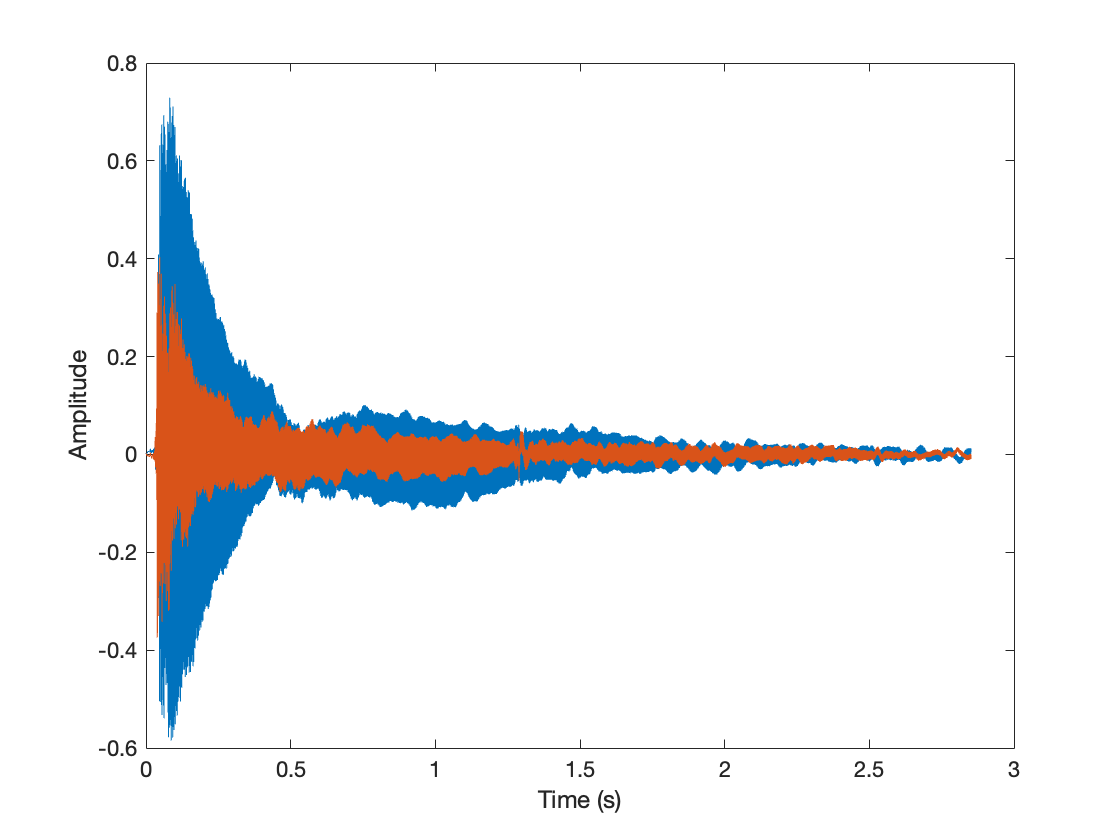
\includegraphics[width = 0.45\textwidth]{signal_before_mean.png}
}
\subfigure[Exemple de signal après moyenner]{
\label{Fig.sub.2}
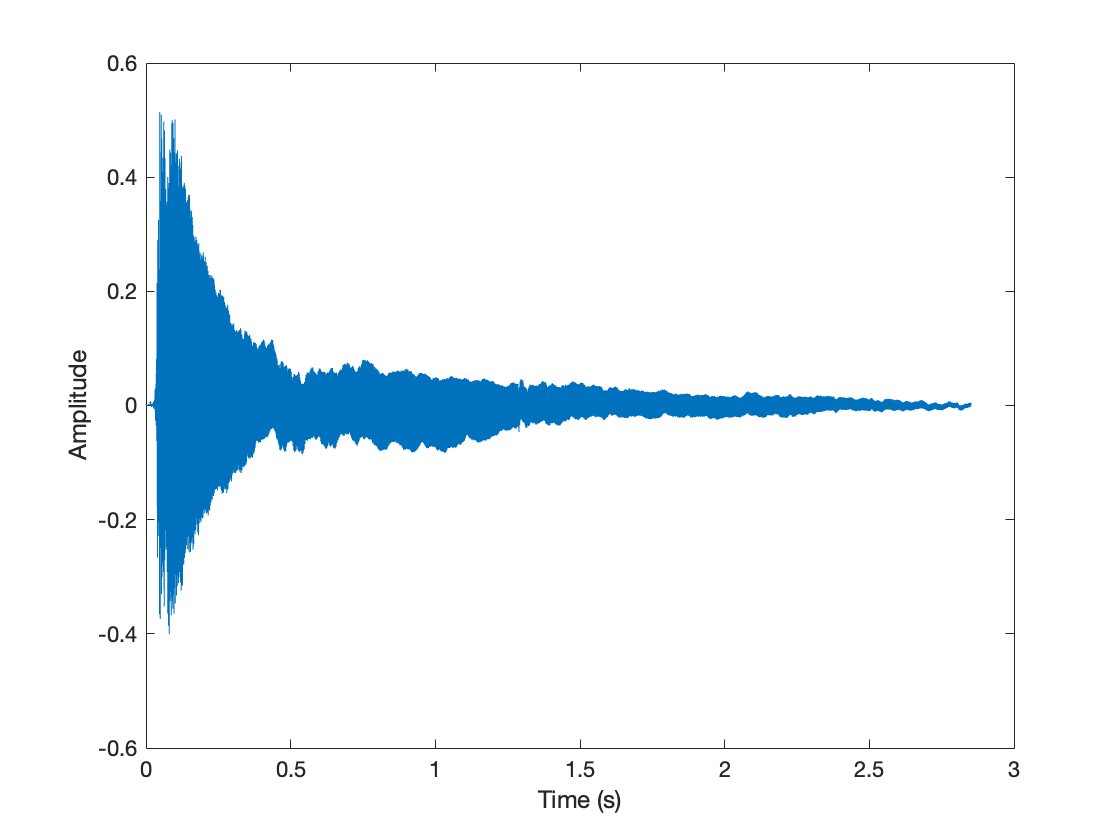
\includegraphics[width = 0.45\textwidth]{signal_after_mean.png}
}
\caption{Exemple de signal}
\label{Fig.main}
    % ici c'est le problem de overleaf que l'image ne marche pas
\end{figure}

\textcolor{blue}{\subsubsection{Acquisition et Pré-traitement du Signal}}

Dans cette première étape, nous chargeons une série de fichiers audio correspondant à différentes notes jouées par des instruments tels que le violon, la flûte et le piano. Ces fichiers audio sont ensuite convertis en signaux mono pour simplifier l'analyse. Pour chaque signal, nous calculons la puissance du signal en utilisant une fenêtre glissante de taille fixe. La puissance ainsi obtenue est ensuite convertie en décibels (dB). Ce processus est essentiel pour préparer le signal en vue de l'analyse ultérieure. 
\textcolor{blue}{\subsubsection{Détection des Notes}}
La détection se fait en trouvant les points où la puissance du signal dépasse un seuil défini (1\% de la puissance maximale). Les indices correspondants sont ensuite convertis en temps, fournissant ainsi les instants de début et de fin de chaque note. Les notes d'une durée inférieure à une seconde sont éliminées pour garantir la qualité des données. 
Fig.\ref{fig:Note_Detection} est le signal avec les notes détectées(partie rouge).
\begin{figure}[htb]
    \centering
    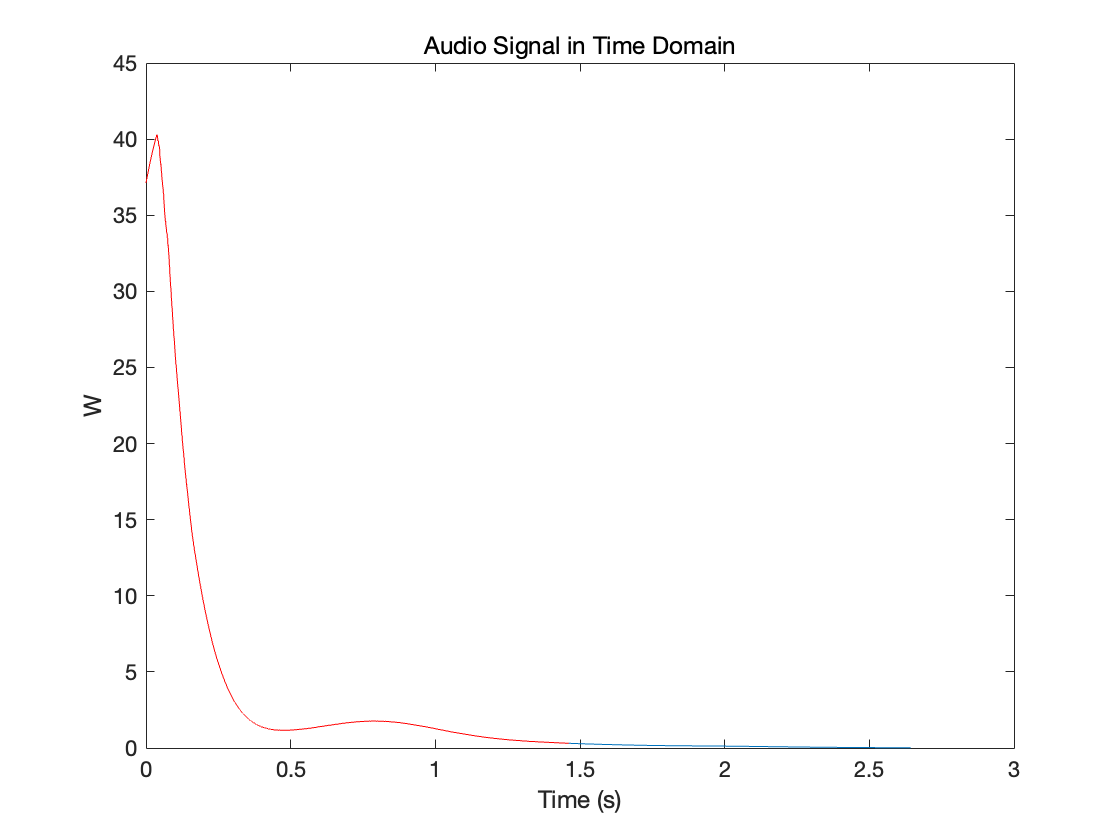
\includegraphics[width=0.8\textwidth]{signal_with_note_detected.png}
    \caption{Exemple signal avec les notes détectées}
    \label{fig:Note_Detection}
\end{figure}
\textcolor{blue}{\subsubsection{Détermination de la Fréquence Fondamentale}}
Le décodage des caractéristiques de chaque note s'effectue en calculant la puissance moyenne, la fréquence fondamentale ($f_0$), la fréquence de la plus haute harmonique ($f_h$), et le nombre d'harmoniques dans la bande de fréquences.La détection précise de la fréquence fondamentale ($f_0$) est essentielle dans l'analyse des signaux sonores, notamment pour l'étude des notes musicales. Ces informations sont extraites à partir du signal audio, utilisant diverses fonctions telles que le calcul de la moyenne de puissance, la fréquence fondamentale par auto-corrélation, et le comptage des harmoniques. Les résultats sont affichés pour chaque note, fournissant une caractérisation détaillée des éléments musicaux contenus chaque fichier audio ainsi que la note et l'octave associée à la fréquence. 

L'ensemble de ces étapes contribue à élaborer un algorithme complet de détection et de caractérisation des notes de musique, avec une option facultative pour estimer la direction de la source sonore sur des signaux acquis par deux micros différents. 

Dans notre étude, nous avons appliqué deux méthodes distinctes pour calculer cette fréquence fondamentale, puis nous les avons comparées afin de vérifier leur exactitude.

La première méthode s'appuie sur la détection de la fréquence qui présente la densité de puissance la plus élevée après avoir effectué une transformation de Fourier rapide (FFT). Cette approche est basée sur l'hypothèse que, dans la majorité des cas, la fréquence fondamentale correspond à la fréquence la plus basse ayant la plus grande densité de puissance.
\begin{equation}
    f_0 = \arg\max_f(\frac{2}{N}|FFT(signal)|)
\end{equation}

Quant à la seconde méthode, nous utilisons le principe de l'auto-corrélation dans le domaine temporel. Cette technique permet de détecter les répétitions périodiques au sein du signal, ce qui facilite l'identification de la fréquence fondamentale, même en présence de harmoniques complexes ou de bruit.
\begin{equation}
    f_0 = \frac{f_s}{Lag_{peak}}
\end{equation}
Où: 
\begin{itemize}
    \item $f_0$ est la fréquence fondamentale  
    \item $f_s$ est la fréquence d'échantillonnage 
    \item $Lag_{peak}$ est le temps de retard correspondant au premier pic significatif de la fonction d'auto-corrélation.
\end{itemize}

Ces méthodes contribuent à élaborer un algorithme complet de détection et de caractérisation des notes de musique. En combinant et en comparant les résultats obtenus par ces deux méthodes, nous pouvons augmenter la fiabilité de notre analyse et assurer une détection plus précise de la fréquence fondamentale, ce qui est crucial pour une compréhension approfondie des propriétés acoustiques des notes analysées.

\textcolor{blue}{\subsubsection{Analyse des Harmoniques}}
Dans l'analyse des signaux audio, la détection précise des harmoniques est essentielle pour comprendre les caractéristiques spectrales du signal.

Notre recherche utilise une méthode basée sur la transformée de Fourier rapide (FFT) pour identifier les composantes harmoniques d'un signal. Ce processus consiste à calculer la FFT du signal et à en extraire les points de fréquence qui répondent à des conditions spécifiques et qui représentent les composantes harmoniques.

Tout d'abord, nous effectuons une FFT sur le signal original pour obtenir son spectre, et nous ne considérons que la partie positive de la fréquence. Dans le spectre, nous identifions d'abord le point de fréquence ayant la puissance la plus élevée (\(P_{max}\)), et à partir de là, un seuil relatif est fixé (typiquement 40 dB en dessous du point de puissance maximale). Tous les points de fréquence supérieurs à ce seuil sont initialement reconnus comme des harmoniques possibles.

Ensuite, pour chaque multiple entier de la fréquence fondamentale (\(n \times f_0 \), où n est un nombre naturel), nous recherchons les points du spectre qui sont les plus proches de ces fréquences. Si les fréquences de ces points ne dépassent pas un seuil de fréquence maximale fixé (\(f_{max}\)) avec une puissance d'au moins 10\% de la puissance maximale, ces points de fréquence sont identifiés comme des harmoniques. De cette manière, nous pouvons extraire efficacement les composants harmoniques du signal.
\begin{equation}
    Harmonics = \{f_n | f_n = n \times f_0, n \in \mathbb{N}, f_n \leq f_{max}, P(f_n) \geq 0.1 \times P_{max} \}
\end{equation}
où :
\begin{itemize}
    \item \(f_n\) est la fréquence de la n-ième harmonique
    \item \(f_0\) est la fréquence fondamentale
    \item \(P(f_n)\) est la densité spectrale de puissance à la fréquence \(f_n\)
    \item \(P_{max}\) est la maxime dans le spectral de fréquence 
    \item \(f_{max}\) est le seuil de fréquence le plus élevé pour la détection des harmoniques
\end{itemize}

\newpage
\textcolor{blue}{\subsection{Résultats Expérimentaux}}
ici est resultats

\newpage
\textcolor{blue}{\subsection{Conclusion}}
En conclusion, nous avons réussi par le code via Matlab à répondre aux attentes du cahier des charges, c'est à dire à caractériser des notes de musiques. Cette caractérisation passe par la détection de la note jouées, de sa fréquence fondamentale et de son harmonique et de sa puissance moyenne en dBm. Le programme détecte aussi les instants de début et de fin ainsi que le nombre d'harmoniques.

Les résultats à l'exécution du programme sont cohérent avec ce que l'on attend (avec le nom des fichiers qui donnent le nom des notes) et aussi de ce l'on entend.
\textcolor{blue}{\section{Chapitre III : Problème IV}}

\end{document}